\chapter{Análisis de los resultados}

En este capítulo se comparan las cuatro rutas evaluadas: la implementación propia en CUDA, la implementación Triton, SDPA y SDPA utilizando el backend de cuDNN. Las métricas de Nsight Compute corresponden a la configuración de perfilado con \(N=8192\), \(d=128\), BF16, \(B=H=1\) y atención no causal. Las medidas temporales se realizan de forma independiente mediante eventos CUDA y 100 repeticiones por longitud de secuencia, utilizando la misma semilla pseudoaleatoria en todas las implementaciones.

El análisis distingue deliberadamente entre \textbf{hechos medidos} y \textbf{hipótesis de interpretación}. Las métricas permiten observar qué ocurre durante la ejecución; cuando se propone una causa que no está demostrada directamente por un contador hardware, se presenta explícitamente como interpretación o línea de investigación.

\section{Kernels observados en SDPA}

En la configuración perfilada, la ruta SDPA que no fuerza cuDNN ejecuta dos kernels principales:

\begin{verbatim}
flash_fwd_splitkv_kernel
flash_fwd_splitkv_combine_kernel
\end{verbatim}

La presencia de ambos kernels es un \textbf{hecho observado} directamente en Nsight Compute. El nombre del primero indica que la implementación utiliza una variante denominada \textit{split-KV}; sin embargo, este trabajo no analiza ni reconstruye el mecanismo interno empleado por PyTorch para realizar esa partición. Para la comparación experimental sólo se retienen dos observaciones directamente medibles: SDPA lanza un número mayor de CTAs que las otras rutas y necesita un segundo kernel de combinación. Cuando se comparan tiempos, el coste de la ruta SDPA debe entenderse como el coste conjunto de los kernels que forman la operación.

\section{Registros y ocupación}

Las Tablas~\ref{tab:register_usage} y~\ref{tab:occupancy_results} separan el consumo de registros de la ocupación para mantener una tipografía legible. El número de \textit{warps} por CTA y la residencia máxima se recogen posteriormente junto con la granularidad de lanzamiento. CUDA presenta el menor número de registros por hilo y la mayor ocupación teórica, pero obtiene la menor ocupación alcanzada.

\begin{table}[H]
\centering
\caption{Uso de registros por hilo para \(N=8192\).}
\label{tab:register_usage}
\begin{tabular}{lrr}
\toprule
\textbf{Impl.} & \textbf{Reg./hilo} & \textbf{Reg. asignados} \\
\midrule
CUDA   & 148 & 152 \\
Triton & 199 & 200 \\
SDPA   & 240 & 240 \\
cuDNN  & 209 & 216 \\
\bottomrule
\end{tabular}
\end{table}

\begin{table}[H]
\centering
\caption{Ocupación teórica y alcanzada para \(N=8192\).}
\label{tab:occupancy_results}
\begin{tabular}{lrr}
\toprule
\textbf{Impl.} & \textbf{Ocup. teórica} & \textbf{Ocup. alcanzada} \\
\midrule
CUDA   & 18.75\% & 7.56\% \\
Triton & 12.50\% & 12.50\% \\
SDPA   & 12.50\% & 11.51\% \\
cuDNN  & 12.50\% & 12.50\% \\
\bottomrule
\end{tabular}
\end{table}

La Tabla~\ref{tab:occupancy_results} muestra que una mayor ocupación teórica no implica automáticamente mayor rendimiento. CUDA podría mantener hasta tres CTAs residentes por SM, pero el perfil registra sólo un 7.56\% de ocupación alcanzada, equivalente a aproximadamente 4.84 \textit{warps} activos por SM.

La ocupación alcanzada no se obtiene simplemente dividiendo el número de CTAs lanzados entre el número de SM. Nsight Compute la calcula a partir de la actividad efectiva de los \textit{warps}. No obstante, el tamaño del \textit{grid} explica por qué CUDA no puede aprovechar la residencia teórica disponible. Para \(N=8192\) se lanzan 128 CTAs sobre 108 SM:

\begin{equation}
\frac{128}{108}\simeq 1.19\ \text{CTA/SM}.
\end{equation}

Por tanto, aunque los recursos permitirían mantener tres CTAs simultáneos, no existe suficiente trabajo en el \textit{grid} para proporcionar tres bloques a cada SM. La Figura~\ref{fig:occupancy_grid} ilustra esta diferencia entre capacidad de residencia y trabajo realmente disponible.

\begin{figure}[H]
\centering
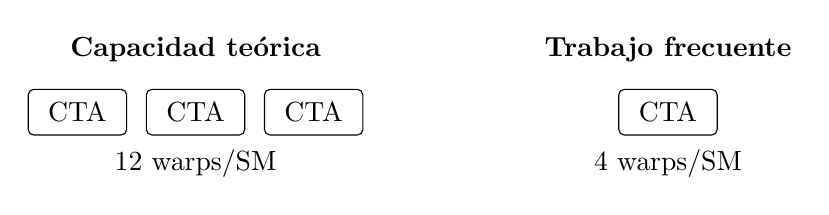
\begin{tikzpicture}[box/.style={draw, rounded corners=2pt, minimum width=1.25cm, minimum height=0.58cm}]
\node at (0,1.8) {\textbf{Capacidad teórica}};
\node[box] at (-1.5,1) {CTA};
\node[box] at (0,1) {CTA};
\node[box] at (1.5,1) {CTA};
\node at (0,0.35) {12 warps/SM};
\node at (6,1.8) {\textbf{Trabajo frecuente}};
\node[box] at (6,1) {CTA};
\node at (6,0.35) {4 warps/SM};
\end{tikzpicture}
\caption{Residencia permitida por recursos frente a trabajo disponible para el kernel CUDA.}
\label{fig:occupancy_grid}
\end{figure}

Triton y el kernel cuDNN perfilado utilizan ocho \textit{warps} por CTA. Aunque sus recursos sólo permiten un CTA residente, ese único bloque ya proporciona ocho \textit{warps} al SM y ambos alcanzan su ocupación teórica. Esta afirmación describe únicamente la configuración observada en el lanzamiento; no reconstruye el \textit{mapping} interno del kernel cuDNN. SDPA utiliza cuatro \textit{warps} por CTA, como CUDA, pero el perfil muestra un \textit{grid} de 384 CTAs y una ocupación alcanzada próxima al máximo permitido por sus recursos.

\section{Memoria compartida y granularidad de lanzamiento}

La Tabla~\ref{tab:launch_smem} muestra que el kernel CUDA tampoco está limitado por un consumo excesivo de memoria compartida. De hecho, utiliza menos memoria compartida por CTA que las demás implementaciones.

\begin{table}[H]
\centering
\caption{Memoria compartida y granularidad de lanzamiento para \(N=8192\).}
\label{tab:launch_smem}
\begin{tabular}{lrrrr}
\toprule
\textbf{Impl.} & \textbf{SMEM/CTA} & \textbf{CTAs} & \textbf{Hilos/CTA} & \textbf{Warps/CTA} \\
\midrule
CUDA   & 32 KiB & 128 & 128 & 4 \\
Triton & 96 KiB & 64  & 256 & 8 \\
SDPA   & 80 KiB & 384 & 128 & 4 \\
cuDNN  & 66 KiB aprox. & 64 & 256 & 8 \\
\bottomrule
\end{tabular}
\end{table}

En CUDA, los cuatro buffers circulares de \(K\) y \(V\) ocupan \(4\times8\,\text{KiB}=32\,\text{KiB}\) por CTA. El perfil puede mostrar además una pequeña cantidad de memoria compartida reservada por el sistema. Los datos de la Tabla~\ref{tab:launch_smem} refuerzan la conclusión anterior: el kernel propio libera recursos suficientes para alojar más CTAs, pero el \textit{grid} no contiene bloques suficientes para explotar esa ventaja en \(N=8192\).

\section{Conflictos de banco}

La Tabla~\ref{tab:bank_conflicts} recoge las métricas de memoria compartida. CUDA y cuDNN no presentan conflictos de banco. En CUDA, este resultado confirma que el patrón de \textit{swizzling} implementado cumple su objetivo.

\begin{table}[H]
\centering
\caption{Conflictos de banco observados en los kernels principales.}
\label{tab:bank_conflicts}
\begin{tabular}{lrrr}
\toprule
\textbf{Impl.} & \textbf{Wavefronts} & \textbf{Conflictos} & \textbf{Conflictos/wavefronts} \\
\midrule
CUDA   & 20\,971\,520 & 0      & 0\% \\
Triton & 21\,053\,440 & 5\,245  & 0.025\% \\
SDPA   & 22\,265\,856 & 23\,284 & 0.105\% \\
cuDNN  & 18\,989\,056 & 0      & 0\% \\
\bottomrule
\end{tabular}
\end{table}

Los conflictos de Triton y SDPA representan una fracción muy pequeña del total de \textit{wavefronts} y no generan \textit{wavefronts} excesivos en estas mediciones. Por ello, no constituyen una explicación convincente de las diferencias de tiempo.

Sí resulta interesante que implementaciones muy optimizadas acepten un número no nulo de conflictos. Una \textbf{hipótesis plausible}, pero no demostrable únicamente con estos contadores, es que eliminar los últimos conflictos podría exigir una disposición de datos, direccionamiento o presión de registros cuyo coste fuese superior a la penalización evitada. Esta observación se mantiene como línea de análisis y no como conclusión atribuida al compilador.

\section{Coalescencia de los accesos globales}

La Tabla~\ref{tab:coalescing} compara los sectores globales solicitados con el número ideal calculado por Nsight Compute. Los cuatro kernels principales presentan el mismo número de sectores reales e ideales.

\begin{table}[H]
\centering
\caption{Sectores globales reales, ideales y excesivos.}
\label{tab:coalescing}
\begin{tabular}{lrrr}
\toprule
\textbf{Impl.} & \textbf{Sectores} & \textbf{Sectores ideales} & \textbf{Excesivos} \\
\midrule
CUDA   & 16\,908\,288 & 16\,908\,288 & 0 \\
Triton & 8\,519\,680  & 8\,519\,680  & 0 \\
SDPA   & 17\,370\,112 & 17\,370\,112 & 0 \\
cuDNN  & 8\,519\,632  & 8\,519\,632  & 0 \\
\bottomrule
\end{tabular}
\end{table}

Por tanto, la coalescencia no explica el orden de rendimiento. En particular, el kernel CUDA no pierde rendimiento por solicitar sectores adicionales debidos a accesos globales mal agrupados. Los sectores analizados en este apartado corresponden a tráfico de datos generado por instrucciones de memoria global; el comportamiento del \textit{frontend} y de la caché de instrucciones se estudia mediante métricas diferentes.

\section{Número total de sectores solicitados}

Aunque todos los kernels sean coalescentes, la cantidad total de sectores solicitados es distinta. La Tabla~\ref{tab:global_sectors} normaliza el tráfico respecto a Triton.

\begin{table}[H]
\centering
\caption{Número total de sectores globales solicitados.}
\label{tab:global_sectors}
\begin{tabular}{lrr}
\toprule
\textbf{Impl.} & \textbf{Sectores} & \textbf{Respecto a Triton} \\
\midrule
Triton & 8\,519\,680  & 1.00$\times$ \\
cuDNN  & 8\,519\,632  & 1.00$\times$ \\
CUDA   & 16\,908\,288 & 1.98$\times$ \\
SDPA   & 17\,370\,112 & 2.04$\times$ \\
\bottomrule
\end{tabular}
\end{table}

Aparecen dos grupos muy claros: Triton y cuDNN solicitan unos 8.52 millones de sectores, mientras que CUDA y SDPA se sitúan alrededor de 17 millones. Este resultado no significa que CUDA acceda peor a memoria; significa que realiza aproximadamente el doble de solicitudes de datos a lo largo de la ejecución. La documentación de cuDNN describe su operación SDPA como una implementación basada en FlashAttention-2 \cite{cudnnAttention}, pero este trabajo no presupone a partir de ello un \textit{mapping} interno concreto.

La implementación propia procesa 16 filas de \(Q\) por \textit{warp} y cuatro \textit{warps} por CTA, es decir, 64 filas de \(Q\) por bloque. El mapping observado para Triton cubre aproximadamente 128 filas de \(Q\) por CTA. La Figura~\ref{fig:reuse_kv} muestra la interpretación utilizada en este trabajo: un bloque mayor de consultas permite amortizar cada tile de \(K,V\) sobre más filas de salida.

\begin{figure}[H]
\centering
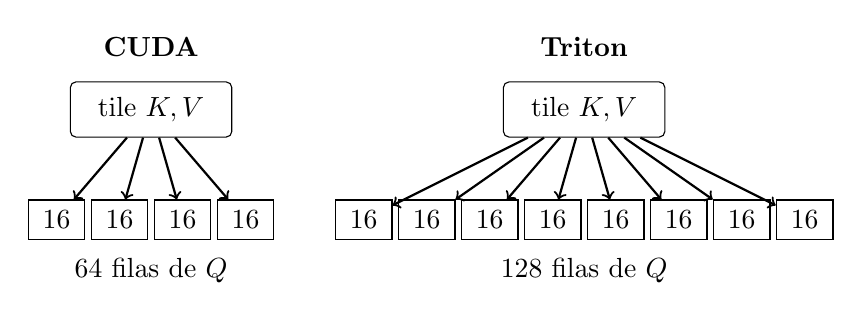
\begin{tikzpicture}[
q/.style={draw, minimum width=0.72cm, minimum height=0.5cm},
kv/.style={draw, rounded corners=2pt, minimum width=2.05cm, minimum height=0.7cm},
arrow/.style={->, thick}
]
\node at (1.5,3.2) {\textbf{CUDA}};
\node[kv] (kvc) at (1.5,2.4) {tile \(K,V\)};
\foreach \x in {0,1,2,3} {\node[q] (c\x) at (0.3+\x*0.8,1) {16};\draw[arrow] (kvc) -- (c\x);}
\node at (1.5,0.35) {64 filas de \(Q\)};
\node at (7,3.2) {\textbf{Triton}};
\node[kv] (kvt) at (7,2.4) {tile \(K,V\)};
\foreach \x in {0,1,2,3,4,5,6,7} {\node[q] (t\x) at (4.2+\x*0.8,1) {16};\draw[arrow] (kvt) -- (t\x);}
\node at (7,0.35) {128 filas de \(Q\)};
\end{tikzpicture}
\caption{Interpretación conceptual de la reutilización de un tile de \(K,V\) sobre las filas de consultas procesadas por un CTA.}
\label{fig:reuse_kv}
\end{figure}

La correspondencia entre un tile mayor de \(Q\) y una mayor reutilización de \(K,V\) es una \textbf{interpretación consistente con las métricas}, no una demostración de que todo el factor dos proceda exclusivamente de esa causa. No obstante, la coincidencia entre el factor de dos en filas de \(Q\) por CTA y el factor aproximado de dos en sectores constituye una evidencia fuerte de que la granularidad global del tile es relevante.

El caso de SDPA es especialmente instructivo: solicita incluso más sectores que CUDA y, aun así, es la ruta más rápida. Por tanto, el número total de sectores no explica por sí solo el rendimiento. El perfil muestra además un número de CTAs considerablemente mayor, por lo que la comparación debe considerar conjuntamente tráfico, reutilización y cantidad de trabajo disponible.

El número de sectores tampoco puede atribuirse al uso de \texttt{\#pragma unroll}. El desenrollado afecta principalmente al código generado y puede aumentar la presión sobre el \textit{frontend} o la caché de instrucciones, pero no convierte por sí solo 8.5 millones de sectores de datos en 16.9 millones.

\section{Actividad de Tensor Cores y jerarquía de memoria}

La Tabla~\ref{tab:tensor_activity} resume varias señales adicionales del perfil. Los porcentajes de actividad Tensor indican que todas las rutas utilizan las unidades matriciales, pero con grados muy diferentes de continuidad.

\begin{table}[H]
\centering
\caption{Actividad aproximada del pipeline Tensor y señales de memoria para \(N=8192\).}
\label{tab:tensor_activity}
\begin{tabular}{lrrr}
\toprule
\textbf{Impl.} & \textbf{Tensor activo} & \textbf{DRAM pico} & \textbf{L2 hit rate} \\
\midrule
CUDA   & 18.1\% & 0.52\% & 97.98\% \\
Triton & 26.4\% & 0.75\% & 95.86\% \\
SDPA   & 57.8\% & 1.73\% & 97.82\% \\
cuDNN  & 38.3\% & 1.09\% & 95.86\% \\
\bottomrule
\end{tabular}
\end{table}

Como se observa en la Tabla~\ref{tab:tensor_activity}, ninguna de las implementaciones se aproxima a saturar el ancho de banda de HBM en este perfil y todas presentan una tasa alta de aciertos en L2. Por ello, los datos no apoyan la hipótesis de que el kernel propio sea simplemente un kernel limitado por ancho de banda de DRAM.

La baja actividad Tensor de CUDA indica, en cambio, que las instrucciones \texttt{mma.sync} no se emiten de forma continua. La estructura del kernel ofrece varias causas compatibles con esta observación: actualizaciones frecuentes del \textit{softmax online}, reducciones escalares, dependencias entre resultados, cargas desde memoria compartida y barreras entre los cuatro \textit{warps} del CTA. Con \(B_c=16\), una secuencia de 8192 elementos requiere

\begin{equation}
\frac{8192}{16}=512
\end{equation}

iteraciones del bucle principal, cada una con cálculo matricial, actualización de normalización y coordinación del pipeline. Se considera por tanto una \textbf{hipótesis respaldada por la estructura del kernel} que parte de la diferencia restante provenga de la dificultad para mantener alimentados los Tensor Cores entre grupos de MMA, especialmente cuando hay pocos \textit{warps} independientes disponibles.

\section{Mediciones temporales}

Las Tablas~\ref{tab:timings_cuda_triton} y~\ref{tab:timings_sdpa_cudnn} recogen las medias y desviaciones típicas obtenidas mediante eventos CUDA. Todas las implementaciones utilizan la misma semilla 0, las mismas dimensiones, BF16 y 100 repeticiones por longitud de secuencia. Se presentan en dos tablas para mantener una tipografía legible.

\begin{table}[H]
\centering
\caption{Tiempo medio y desviación típica de CUDA y Triton (ms).}
\label{tab:timings_cuda_triton}
\begin{tabular}{rrr}
\toprule
\textbf{\(N\)} & \textbf{CUDA} & \textbf{Triton} \\
\midrule
8\,192       & 0.579 $\pm$ 0.002 & 0.467 $\pm$ 0.007 \\
16\,384      & 1.633 $\pm$ 0.032 & 1.702 $\pm$ 0.004 \\
32\,768      & 5.654 $\pm$ 0.061 & 5.235 $\pm$ 0.028 \\
65\,536      & 22.243 $\pm$ 0.185 & 18.122 $\pm$ 0.091 \\
131\,072     & 85.192 $\pm$ 0.279 & 72.471 $\pm$ 0.356 \\
262\,144     & 341.337 $\pm$ 1.500 & 278.601 $\pm$ 0.054 \\
524\,288     & 1380.594 $\pm$ 7.278 & 1113.618 $\pm$ 0.221 \\
1\,048\,576 & 5576.997 $\pm$ 15.101 & 4453.727 $\pm$ 3.102 \\
\bottomrule
\end{tabular}
\end{table}

\begin{table}[H]
\centering
\caption{Tiempo medio y desviación típica de SDPA y cuDNN (ms).}
\label{tab:timings_sdpa_cudnn}
\begin{tabular}{rrr}
\toprule
\textbf{\(N\)} & \textbf{SDPA} & \textbf{cuDNN} \\
\midrule
8\,192       & 0.252 $\pm$ 0.020 & 0.317 $\pm$ 0.005 \\
16\,384      & 1.163 $\pm$ 0.018 & 1.204 $\pm$ 0.021 \\
32\,768      & 3.783 $\pm$ 0.071 & 3.840 $\pm$ 0.108 \\
65\,536      & 13.148 $\pm$ 0.116 & 13.506 $\pm$ 0.213 \\
131\,072     & 52.172 $\pm$ 0.299 & 54.304 $\pm$ 0.312 \\
262\,144     & 199.515 $\pm$ 0.411 & 207.784 $\pm$ 0.020 \\
524\,288     & 795.068 $\pm$ 0.370 & 830.797 $\pm$ 0.121 \\
1\,048\,576 & 3176.341 $\pm$ 3.635 & 3370.064 $\pm$ 4.832 \\
\bottomrule
\end{tabular}
\end{table}

La Figura~\ref{fig:timing_lines} representa directamente la longitud de secuencia frente al tiempo medio de ejecución. El eje horizontal utiliza escala logarítmica en base 2 para separar uniformemente las longitudes ensayadas, que son potencias de dos, mientras que el eje vertical se mantiene \textbf{lineal} en milisegundos. De esta forma, la distancia vertical entre las curvas conserva la diferencia absoluta de tiempo y resulta más visible la separación entre CUDA y las rutas de referencia para secuencias grandes.

\clearpage
\begin{figure}[p]
\centering
\definecolor{cudaColor}{RGB}{31,119,180}
\definecolor{tritonColor}{RGB}{255,127,14}
\definecolor{sdpaColor}{RGB}{44,160,44}
\definecolor{cudnnColor}{RGB}{214,39,40}
\begin{tikzpicture}
\begin{semilogxaxis}[
    width=0.94\textwidth,
    height=0.72\textheight,
    xlabel={Longitud de secuencia \(N\)},
    ylabel={Tiempo medio (ms)},
    log basis x=2,
    ymin=0,
    ymax=6000,
    ytick={0,1000,2000,3000,4000,5000,6000},
    grid=both,
    major grid style={line width=.4pt},
    minor grid style={line width=.2pt},
    legend style={at={(0.5,-0.12)}, anchor=north, legend columns=4, font=\normalsize},
    legend cell align=left,
    xtick={8192,16384,32768,65536,131072,262144,524288,1048576},
    xticklabels={8K,16K,32K,64K,128K,256K,512K,1M},
    tick label style={font=\normalsize},
    label style={font=\large},
    line width=1.2pt,
    mark size=3pt
]
\addplot[color=cudaColor,mark=*,very thick] coordinates {
(8192,0.578509) (16384,1.632676) (32768,5.654231) (65536,22.243174)
(131072,85.192307) (262144,341.336761) (524288,1380.593872) (1048576,5576.997070)};
\addlegendentry{CUDA}
\addplot[color=tritonColor,mark=square*,very thick] coordinates {
(8192,0.466913) (16384,1.701990) (32768,5.234739) (65536,18.122097)
(131072,72.470833) (262144,278.600891) (524288,1113.617798) (1048576,4453.726563)};
\addlegendentry{Triton}
\addplot[color=sdpaColor,mark=triangle*,very thick] coordinates {
(8192,0.251556) (16384,1.163203) (32768,3.783373) (65536,13.148180)
(131072,52.171963) (262144,199.515289) (524288,795.067566) (1048576,3176.340576)};
\addlegendentry{SDPA}
\addplot[color=cudnnColor,mark=diamond*,very thick] coordinates {
(8192,0.317102) (16384,1.203753) (32768,3.840185) (65536,13.505505)
(131072,54.303654) (262144,207.783890) (524288,830.796509) (1048576,3370.063965)};
\addlegendentry{cuDNN}
\end{semilogxaxis}
\end{tikzpicture}
\caption{Tiempo medio de ejecución frente a longitud de secuencia, con eje vertical lineal.}
\label{fig:timing_lines}
\end{figure}
\clearpage

Para \(N=8192\), SDPA es aproximadamente

\begin{equation}
\frac{0.579}{0.252}\simeq 2.30\times
\end{equation}

más rápido que CUDA. Para \(N=1\,048\,576\), la relación se reduce a

\begin{equation}
\frac{5576.997}{3176.341}\simeq 1.76\times.
\end{equation}

La reducción del factor al aumentar \(N\) es coherente con la hipótesis de que una parte importante de la penalización para \(N=8192\) procede de la falta de bloques suficientes para poblar la A100. Cuando \(N\) es muy grande, el \textit{grid} deja de ser escaso y permanece una diferencia asociada a la eficiencia sostenida dentro del SM.

Triton estabiliza una ventaja menor sobre CUDA para tamaños grandes: aproximadamente \(1.225\times\), \(1.240\times\) y \(1.252\times\) para 256K, 512K y 1M, respectivamente. Además, en \(N=16384\) CUDA es ligeramente más rápida que Triton (1.633 ms frente a 1.702 ms), lo que confirma que no existe un único orden de rendimiento para todos los tamaños.

\section{Escalabilidad y throughput sostenido}

A partir de aproximadamente \(N=65536\), duplicar la longitud de secuencia multiplica el tiempo por un factor cercano a cuatro en las cuatro rutas. Este comportamiento concuerda con el coste cuadrático de la atención exacta:

\begin{equation}
T(N)\propto N^2.
\end{equation}

Considerando aproximadamente \(4N^2d\) operaciones de coma flotante para los productos \(QK^T\) y \(PV\), con \(d=128\), se obtiene el throughput sostenido aproximado de la Tabla~\ref{tab:tflops_results}.

\begin{table}[H]
\centering
\caption{Throughput aproximado en el régimen de secuencias grandes.}
\label{tab:tflops_results}
\begin{tabular}{lr}
\toprule
\textbf{Impl.} & \textbf{Throughput aproximado} \\
\midrule
CUDA   & 101 TFLOP/s \\
Triton & 126 TFLOP/s \\
cuDNN  & 167 TFLOP/s \\
SDPA   & 177 TFLOP/s \\
\bottomrule
\end{tabular}
\end{table}

La Tabla~\ref{tab:tflops_results} permite separar dos efectos. Para \(N=8192\), CUDA sufre simultáneamente por la cantidad limitada de trabajo global y por su eficiencia interna. En secuencias grandes existe trabajo suficiente para todos los SM y la diferencia restante se aproxima más a la eficiencia sostenida del kernel. El kernel propio se estabiliza alrededor de 100 TFLOP/s, mientras que Triton se sitúa en torno a 126 TFLOP/s y las rutas de biblioteca alcanzan valores mayores.

\section{Lecciones aprendidas y posibles mejoras}

Los perfiles muestran que una parte importante del trabajo de optimización de bajo nivel produjo el efecto buscado. En CUDA no aparecen sectores excesivos por falta de coalescencia, no hay conflictos de banco, no se observa \textit{register spilling} y el consumo de registros y memoria compartida es inferior al de varias alternativas. Estas son mejoras reales y medibles.

La principal limitación se encuentra en un nivel superior de diseño. El kernel propio procesa 64 filas de \(Q\) por CTA y recorre \(K,V\) con un tile físico de 16 filas. Frente a Triton, cuyo \textit{mapping} generado permite identificar un bloque de consultas mayor, esta configuración obtiene menor reutilización de \(K,V\). En cuDNN no se reconstruye el \textit{mapping} interno: el menor número de sectores solicitado es únicamente \textbf{consistente con una mayor reutilización efectiva}, no una demostración de un tamaño de tile concreto. Para el tamaño perfilado, CUDA también expone menos trabajo global que la ruta SDPA. En otras palabras, se optimizó intensamente una granularidad local que no era necesariamente la mejor granularidad global para una A100 con 108 SM.

Las líneas de mejora que se desprenden de los resultados son:

\begin{enumerate}
    \item aumentar el número de filas de \(Q\) procesadas por CTA para reutilizar cada tile de \(K,V\) sobre más consultas;
    \item estudiar una reorganización donde parte de \(Q\) se mantenga en memoria compartida si ello permite aumentar el tile sin disparar el consumo de registros;
    \item agrupar varias iteraciones físicas de 16 filas de \(K,V\) antes de actualizar el \textit{softmax online}, reduciendo la frecuencia de reescalados y sincronizaciones;
    \item reducir la frecuencia o el alcance de las barreras entre \textit{warps};
    \item explorar estrategias de partición que incrementen el paralelismo global en secuencias donde el número de CTAs resulta insuficiente.
\end{enumerate}

La conclusión principal no es que una optimización concreta haya sido incorrecta, sino que el rendimiento final depende del equilibrio entre reutilización de datos, paralelismo, sincronización y capacidad para mantener alimentadas las unidades de ejecución. Un kernel puede presentar accesos coalescentes, cero conflictos de banco y bajo consumo de recursos y, aun así, quedar por detrás si la distribución global del trabajo no aprovecha adecuadamente el dispositivo.
